\providecommand{\main}{..}
\documentclass[\main/main.tex]{subfiles}


\begin{document}


\section{Markov chains} \label{markov_chain}
A Markov chain (MC) is a special type of stochastic processes  $  \{ X_t, t \in T\}$ where $X_{t+1}$ depends on $X_{t}$ only, i.e. \lq\lq the probability of the next random outcome depends on the present realisation but it is independent of the past'' \citep{Grinstead1997}. 
This means that, given the present state of the random process, the conditional probability of the next state depends on the present state but it is independent of previous states.\\
In other words, \lq\lq only the most recent point in the trajectory affects what happens next'' \citep{Holmes2015}. More formally, a Markov chain is defined as \lq\lq an indexed sequence of random variables, $\{X_0, X_1, X_2, ...\}$ that satisfies the Markov property'' \citep{Sheskin2010}:

\begin{equation}
\begin{split}
     & \mathds{P} \big(X_{t+1} = s |X_t = s_t, X_{t-1} = s_{t-1}, . . . , X_0 = s_0\big) = 
     \mathds{P} \big(X_{t+1} = s |X_t = s_t\big)\\
    & \text{for all} \; t = 1, 2, 3, ... \; \text{and for all states} \; s_0, s_1, . . . , s_t, s.\\
\end{split}
\end{equation}\\



Usually $t$ usually denotes time, meaning that, at every time $t$ in the set $T$, a realisation of the random variable $X_t$ is observed.
Some authors use an equivalent notation $\{X_n, n \in N\}$, where the index $t$ is replaced by $n$.\\


Markov chain models were introduced in the early 20th century by the Russian mathematician A. A. Markov \citep{Hayes2013}. In the United States, these models began to gain popularity from the 1950's, when both academia - see for instance, \cite{Feller1950}, \cite{Howard1960}, and \cite{Kemeny1960} - and mathematicians at the RAND Corporation in California started investigating theory and applications of Markov decision processes \citep{Sheskin2010}. Markov chains have now been applied to a variety of problems such as Markovian queueing systems, webpage ranking, inventory control, customer lifetime value etc. \cite{Ching2006} provide an overview and some practical examples of the many fields of application of such models.\\
See instead \cite{Karlin1975} for a detailed discussion of stochastic process and Markov chains. \\



\subsubsection{Main concepts and definitions}

Just to mention some essential terminology, we say that a Markov chain can assume any value, called \textit{state}, inside the \textit{state space}, with $S \subseteq \mathds{R}$. In the context of this analysis, we consider finite and mutually exclusive states $S = \{s_1,s_2,...,s_t, s\}$ in which the Markov chain is observed. For instance, if $X_t = s_i$ we say that the Markov chain, or process, is in state $s_i$ at time $t$.\\
If the set $S$ is finite or countable, the state space is said to be \textit{discrete}, otherwise it is said to be \textit{continuous}. A further distinction is made between \textit{discrete-time} Markov chains and \textit{continuous-time} ones. In the former, the set $T$ is finite or countable, i.e. $T = \{ 0,1,2,..\}$ while in the latter $T$ is not finite or countable, i.e $T = [0,\infty)$, or $T = [0,K]$ for some K. In this case $X_t$ is allowed to change at every instant in time \citep{Holmes2015}.



The \textit{trajectory}, or \textit{sample path}, will be the set of values that the sequence of random variables assumes over a given time horizon. For instance, when we observe $X_0 = s_0, X_1 = s_1, X_2 = s_2, ...$, we say that the Markov chain has trajectory $s_0, s_1, s_2,...$. 

The sequence of random variables is typically observed at equally spaced points in time, called 
\textit{epochs}. An epoch is denoted by $t = 0, 1, 2, ...$ . Epoch $t$ designates the end of time period $t$ and the beginning of period $t + 1$. The time interval between two successive epochs is called \textit{period or step}. \citep{Sheskin2010}.\\


\begin{figure}[H]
\centering
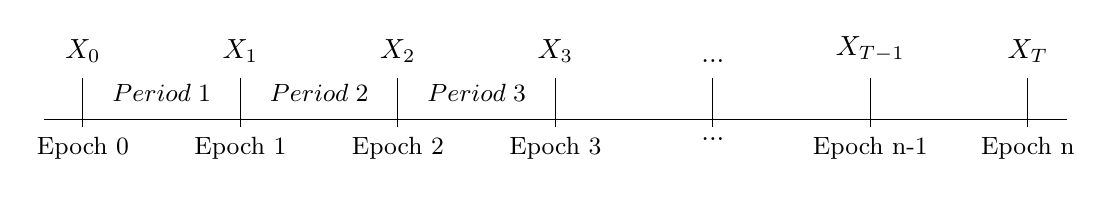
\begin{tikzpicture}
% draw horizontal line   
\draw (-0.5,0) -- (12.5,0);
% draw vertical lines
\foreach \x in {0,2,4,6,8,10,12}
\draw (\x cm,15pt) -- (\x cm,-3pt);
% draw nodes
\draw (0,0) node[below=3pt] {\small Epoch  0} node[above=3pt] {$   $};
\draw (0,0) node[above=17pt] {$X_0$} node[above=3pt] {};
\draw (2,0) node[above=17pt] {$X_1$} node[above=3pt] {};
\draw (4,0) node[above=17pt] {$X_2$} node[above=3pt] {};
\draw (6,0) node[above=17pt] {$X_3$} node[above=3pt] {};
\draw (8,0) node[above=17pt] {$...$} node[above=3pt] {};
\draw (10,0) node[above=17pt] {$X_{T-1}$} node[above=3pt] {};
\draw (12,0) node[above=17pt] {$X_{T}$} node[above=3pt] {};
\draw (1,0) node[below=3pt] {} node[above=3pt] {\small $Period \; 1$};
\draw (2,0) node[below=3pt] { \small Epoch 1} node[above=3pt] {};
\draw (3,0) node[below=3pt] {$  $} node[above=3pt] {\small $Period \; 2$};
\draw (4,0) node[below=3pt] {\small Epoch 2} node[above=3pt] {};
\draw (5,0) node[below=3pt] {} node[above=3pt] {\small $Period \; 3$};
\draw (6,0) node[below=3pt] {\small Epoch 3} node[above=3pt] {$  $};
\draw (8,0) node[below=3pt] {$...$} node[above=3pt] {$  $};
\draw (10,0) node[below=3pt] {\small Epoch n-1} node[above=3pt] {$  $};
\draw (12,0) node[below=3pt] {\small Epoch n} node[above=3pt] {$  $};
\end{tikzpicture}
\caption{Epochs and time periods of a Markov chain}
\label{fig:markov_chain}
\end{figure}







Clearly, this is one of the simplest form of dependency \citep{Sheskin2010}. 




\subsubsection{How to describe a Markov chain}

Markov chains can be describes through \textit{transition diagrams} or \textit{transition matrices}.

A transition diagram visually represents a Markov chain using nodes for states and directed links for the probability of moving from one state to another \citep{Gagniuc2017}. 

A transition matrix collects the transition probabilities $p_{ij}$ and it is usually indicated by the capital letter $\mathbf{P}$. 
Much of the literature on Markov chains considers row-stochasticity (i.e. the probabilities on each row of the matrix sum to 1). However, there are authors that prefer setting matrices as column-stochastic, see for example \cite{Caswell2006}. In this context, we will adopt Caswell's formulation and consider a transition matrix $\mathbf{P}$ of the form:


\begin{center}
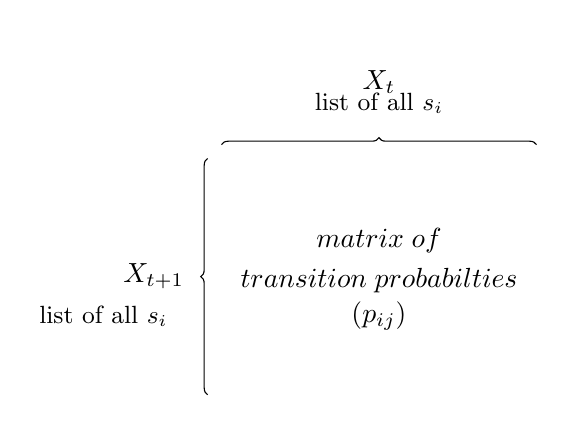
\begin{tikzpicture}
\node[circle,label={$matrix\; of$}] at (2,1.5) {};
\node[circle,label={$transition \; probabilties$}] at (2,1) {};
\node[circle] at (2,1) {$(p_{ij})$};
\node[circle] at (2,3.7) {\small list of all $s_i$};
\node[circle] at (-1.5,1) {\small list of all $s_i$};
\draw[decoration={brace,raise=5pt},decorate]
  (0,0) -- node[left=10pt] {$X_{t+1}$} (0,3);
\draw[decoration={brace,raise=5pt},decorate]
  (0,3) -- node[above=20pt] {$X_t$} (4,3);
\end{tikzpicture}
\end{center}







\subsubsection{The transition probabilities of a transition matrix}
In order to compute the transition probabilities of a Markov chain, we can imagine the process starting in state $i$ and then moving in steps through the other states. The following explanation is taken from \cite{Sheskin2010}, \cite{Howard1960}, and \cite{Holmes2015}. \\

Let $\mathds{P}(X_t = i)$ be the probability that the Markov chain is in state $i$ at epoch $t$ and let $\mathds{P}(X_{t+1} = j)$ be the probability that the Markov chain will be in state $j$ in the next epoch $t+1$. Define $\mathds{P}(X_{t+1}
= j|X_{t} = i)$ as the conditional probability of the Markov chain. i.e. the probability that the process will be in state $j$ at epoch $t + 1$, given that it is in state $i$ at epoch $t$. 
This conditional probability is called the \textit{transition probability} and it is alternatively denoted by $p_{ij}$ \citep{Sheskin2010}. Note that $p_{ij}$  refers to the the probability of moving from state $i$ to state $j$ in \textit{one step}:

\begin{equation}
    p_{ij} = \mathds{P}(X_{t+1} = j |X_t = i) \; \; \text{for}\; \; i,j \in S, \; \; t=0,1,2,...
\end{equation}
Without loss of generality, assume that the state space has $N$ elements, $S=\{1,2,...,N\} $. Clearly, since the Markov chain must be in some state at time $t+1$ we have \citep{Howard1960}:
\begin{equation}
 \sum_{j=1}^N     p_{ij} = 1
\end{equation}
 Moreover, the $p_{ij}$ are probabilities and therefore:
\begin{equation}
 0 \leq p_{ij} \leq 1
\end{equation}\\

A typical assumption that one could make is that the transition probabilities are \textit{stationary} over time (or \textit{time homogeneous)} meaning that they do not change over time \citep{Sheskin2010}. If this is the case, it follows that:
\begin{equation}
    p_{ij} = \mathds{P}(X_{t+1} = j |X_t = i)  = \; \; \mathds{P}(X_{0} = j |X_1 = i)
\end{equation}\\


\subsubsection{Transition probabilities of a trajectory}

\noindent As we have seen, Markov chains evolve over time and \lq\lq visit'' a sequence of states, thereby originating a \lq\lq trajectory''. The probability of such trajectory, e.g. $X_0 = a, X_1 = b, X_2 = c$ is a joint probability that can be computed taking into account the Markov property:

\begin{equation}
\begin{split}
   &\mathds{P}(X_0 = a, X_1 = b, X_2 = c) =\\
   =\;  &\mathds{P}(X_0 = a) \mathds{P}(X_1 = b |X_0 = a ) \mathds{P}(X_2 = c |X_1 = b ) = \\
   =\; &p_a \; p_{ab}\; p_{bc}
\end{split}
\end{equation}
where $p_a$ represent the probability that the initial state is equal to $a$. Since the initial state is usually known $p_a = 1$, the above formula simplifies:
\begin{equation}
\begin{split}
   &\mathds{P}(X_0 = a, X_1 = b, X_2 = c) =\\
   =\; &p_{ab}\; p_{bc}
\end{split}
\end{equation}\\


\subsubsection{One-step transition probabilities}
\noindent The one-step transition probabilities represent the probability of making a transition from state $i$ to state $j$ in a one single step. By definition, they are the entries $p_{ij}$ of the matrix $\mathbf{P}$:



\begin{equation}
   \mathds{P} = \Big([ p_{ij}] \Big)
\end{equation}
where
\begin{equation}
    p_{ij} = \mathds{P} ( X_{t+1} = j | X_t = i)
\end{equation}\\


\subsubsection{Two-step transition probabilities}

\noindent The two-step transition probabilities $p_{ij}^2$ represent the probability of making a transition from state $i$ to state $j$ in two steps. To calculate a two-step transition probability one can reason as follows \citep{Sheskin2010}: $p_{ij}^2$ is the conditional probability of going from state $j$ to state $i$ in two steps, i.e. passing through an intermediate state $k$, where $k$ can be any of the states of the Markov chain. Thus, the $p_{ij}^2$ can be computed as the product of a first and second transition probability: the first transition is from state $i$ to state $k$ and the second is from state $k$ to $j$. Since the value of $k$ is unknown, we have sum over all the possible state of $k$. This idea relies on the law of total probability . See \cite{Zwillinger2000} for further details.

To make a simple example, suppose the state space of the Markov chain is $S = \{ 1,2,3\}$. Then, we have:

\begin{equation}
    p_{ij}^2 = p_{i1}p_{1j} + p_{i2}p_{2j} + p_{i3}p_{3j} = \sum_k p_{ik}p_{kj}
\end{equation}

\noindent The two-step transition probabilities are collected in the matrix $\mathbf{P}^{(2)}$. By the rules of matrix multiplication,  $\mathbf{P}^{(2)}$ can be obtained by multiplying the one-step transition matrix by itself:
\begin{equation}
    \mathbf{P}^{(2)} = \mathbf{P} \mathbf{P} = \mathbf{P}^2 
\end{equation}\\
indeed:
\begin{equation}
\begin{split}
  \mathbf{P}^2 = \mathbf{P} \mathbf{P} &= 
\begin{bmatrix}
p_{11} & p_{21} & p_{31} \\
p_{12} & p_{22} & p_{32}  \\
p_{13} & p_{23} & p_{33}  \\
\end{bmatrix}
\begin{bmatrix}
p_{11} & p_{21} & p_{31} \\
p_{12} & p_{22} & p_{32}  \\
p_{13} & p_{23} & p_{33}  \\
\end{bmatrix}=\\
&= 
\begin{bmatrix}
p_{11}p_{11} + p_{21}p_{12} + p_{31}p_{13} & \cdots \\
\vdots\\
\end{bmatrix} =
\begin{bmatrix}
p_{11}p_{11} + p_{12}p_{21} + p_{13}p_{31} & \cdots \\
\vdots\\
\end{bmatrix} =\\
&= 
\begin{bmatrix}
\sum_{k=1}^3 p_{1k}p_{k1} & \cdots\\
\vdots\\
\end{bmatrix} = 
\begin{bmatrix}
\sum_{k=1}^N p_{ik}p_{kj} & \cdots\\
\vdots\\
\end{bmatrix} = 
\mathbf{P}^{(2)} 
\end{split}
\end{equation}\\




\subsubsection{T-step transition probabilities }

The idea for the two-step transition matrix can be shown to extend to the more general case (see \citep{Sheskin2010} or \cite{Holmes2015} for a proof). Hence, the t-step transition matrix is obtained as the  $t^{th}$ power the one-step transition matrix:

\begin{equation}
    \mathbf{P}^{(t)} = \mathbf{P}^t
\end{equation}




\end{document}



